\documentclass{standalone}
\usepackage{tikz}
\usetikzlibrary{patterns, positioning}
\usepackage[sfdefault]{ClearSans} %% option 'sfdefault' activates Clear Sans as the default text font
\usepackage[T1]{fontenc}

\begin{document}
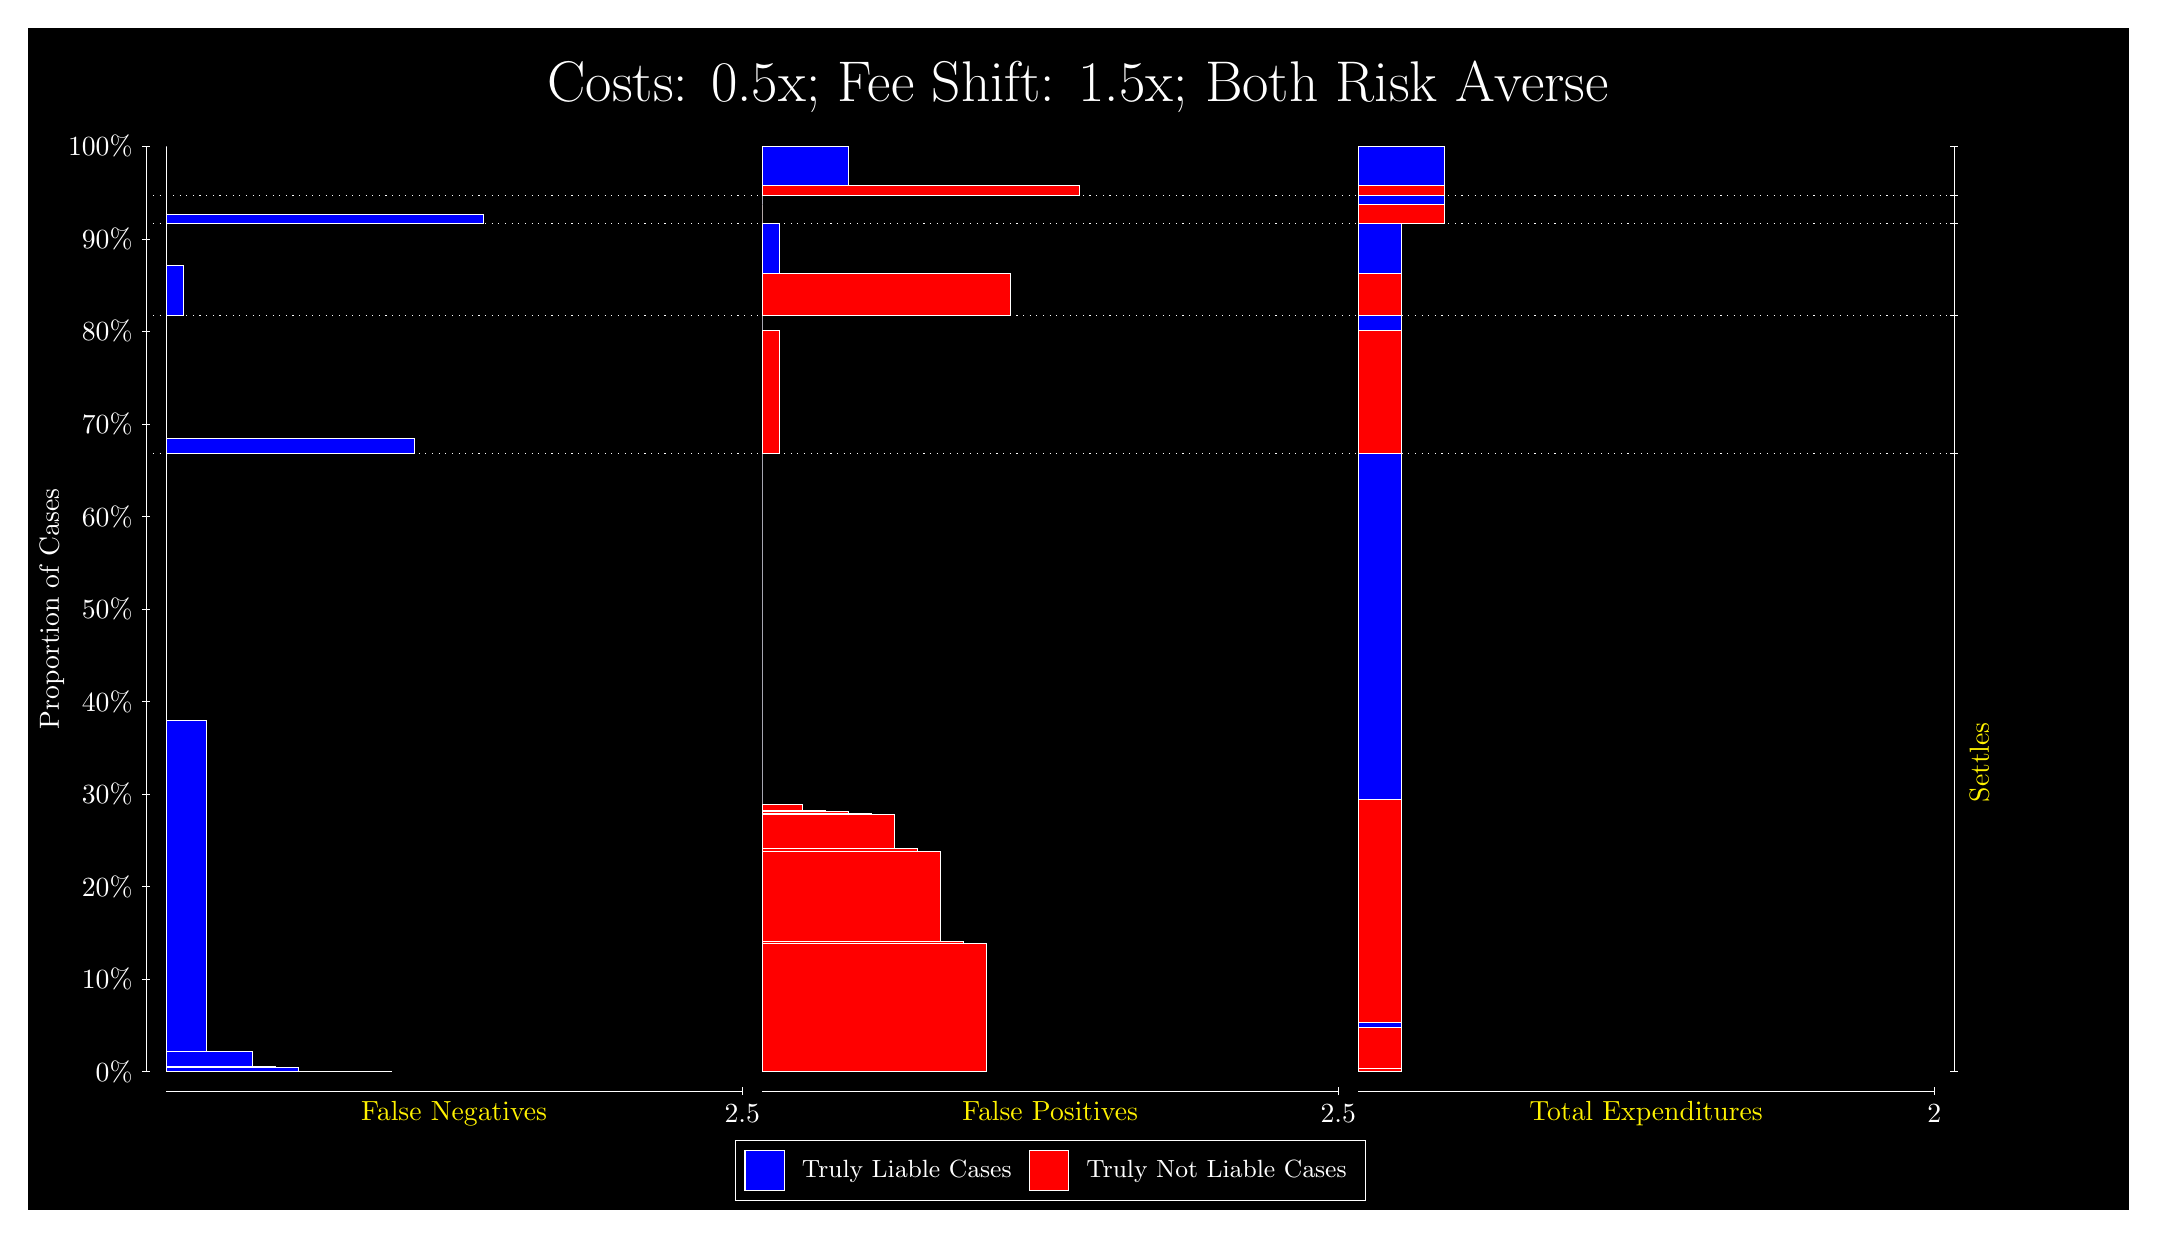
\begin{tikzpicture}
\draw[fill=black] (0,0) rectangle (26.667,15);
\draw[text=white] (0,13.5) rectangle (26.667,15) node[midway] {\huge Costs: 0.5x; Fee Shift: 1.5x; Both Risk Averse};
\draw[white, very thin] (1.5,1.75) -- (1.5,13.5);
\node[rotate=90, text=white, anchor=center] at (0.3, 7.625) {Proportion of Cases};
\draw[white, very thin] (1.45,1.75) -- (1.55,1.75);
\node[text=white, anchor=east] at (1.45, 1.75) {0\%};
\draw[white, very thin] (1.45,2.925) -- (1.55,2.925);
\node[text=white, anchor=east] at (1.45, 2.925) {10\%};
\draw[white, very thin] (1.45,4.1) -- (1.55,4.1);
\node[text=white, anchor=east] at (1.45, 4.1) {20\%};
\draw[white, very thin] (1.45,5.275) -- (1.55,5.275);
\node[text=white, anchor=east] at (1.45, 5.275) {30\%};
\draw[white, very thin] (1.45,6.45) -- (1.55,6.45);
\node[text=white, anchor=east] at (1.45, 6.45) {40\%};
\draw[white, very thin] (1.45,7.625) -- (1.55,7.625);
\node[text=white, anchor=east] at (1.45, 7.625) {50\%};
\draw[white, very thin] (1.45,8.8) -- (1.55,8.8);
\node[text=white, anchor=east] at (1.45, 8.8) {60\%};
\draw[white, very thin] (1.45,9.975) -- (1.55,9.975);
\node[text=white, anchor=east] at (1.45, 9.975) {70\%};
\draw[white, very thin] (1.45,11.15) -- (1.55,11.15);
\node[text=white, anchor=east] at (1.45, 11.15) {80\%};
\draw[white, very thin] (1.45,12.325) -- (1.55,12.325);
\node[text=white, anchor=east] at (1.45, 12.325) {90\%};
\draw[white, very thin] (1.45,13.5) -- (1.55,13.5);
\node[text=white, anchor=east] at (1.45, 13.5) {100\%};

\draw[white, very thin] (24.457,1.75) -- (24.457,13.5);
\draw[white, very thin] (24.407,1.75) -- (24.507,1.75);
\node[anchor=west] at (24.407, 1.75) {};
\draw[white, very thin] (24.407,9.604) -- (24.507,9.604);
\node[anchor=west] at (24.407, 9.604) {};
\draw[white, very thin] (24.407,11.354) -- (24.507,11.354);
\node[anchor=west] at (24.407, 11.354) {};
\draw[white, very thin] (24.407,12.523) -- (24.507,12.523);
\node[anchor=west] at (24.407, 12.523) {};
\draw[white, very thin] (24.407,12.873) -- (24.507,12.873);
\node[anchor=west] at (24.407, 12.873) {};
\draw[white, very thin] (24.407,13.5) -- (24.507,13.5);
\node[anchor=west] at (24.407, 13.5) {};

\draw[white, very thin, fill=blue] (1.75,1.75) rectangle (4.6044,1.7546);
\draw[white, very thin, fill=blue] (1.75,1.7546) rectangle (4.3116,1.755);
\draw[white, very thin, fill=blue] (1.75,1.755) rectangle (4.0188,1.7568);
\draw[white, very thin, fill=blue] (1.75,1.7568) rectangle (3.7261,1.7572);
\draw[white, very thin, fill=blue] (1.75,1.7572) rectangle (3.4333,1.8096);
\draw[white, very thin, fill=blue] (1.75,1.8096) rectangle (3.1406,1.8139);
\draw[white, very thin, fill=blue] (1.75,1.8139) rectangle (2.8478,2.0085);
\draw[white, very thin, fill=blue] (1.75,2.0085) rectangle (2.5551,2.0098);
\draw[white, very thin, fill=blue] (1.75,2.0098) rectangle (2.2623,6.2084);
\draw[white, very thin, fill=red] (1.75,6.2084) rectangle (1.75,9.604);
\draw[white, very thin, fill=blue] (1.75,9.604) rectangle (4.8971,9.7902);
\draw[white, very thin, fill=red] (1.75,9.7902) rectangle (1.75,11.354);
\draw[white, very thin, fill=blue] (1.75,11.354) rectangle (1.9696,11.986);
\draw[white, very thin, fill=red] (1.75,11.986) rectangle (1.75,12.523);
\draw[white, very thin, fill=blue] (1.75,12.523) rectangle (5.7754,12.632);
\draw[white, very thin, fill=red] (1.75,12.632) rectangle (1.75,12.873);
\draw[white, very thin, fill=red] (1.75,12.873) rectangle (1.75,13.011);
\draw[white, very thin, fill=blue] (1.75,13.011) rectangle (1.75,13.5);
\draw[white, very thin, fill=red] (9.3189,1.75) rectangle (12.173,3.381);
\draw[white, very thin, fill=red] (9.3189,3.381) rectangle (11.88,3.4006);
\draw[white, very thin, fill=red] (9.3189,3.4006) rectangle (11.588,4.5454);
\draw[white, very thin, fill=red] (9.3189,4.5454) rectangle (11.295,4.586);
\draw[white, very thin, fill=red] (9.3189,4.586) rectangle (11.002,5.022);
\draw[white, very thin, fill=red] (9.3189,5.022) rectangle (10.709,5.0281);
\draw[white, very thin, fill=red] (9.3189,5.0281) rectangle (10.709,5.0299);
\draw[white, very thin, fill=red] (9.3189,5.0299) rectangle (10.417,5.0585);
\draw[white, very thin, fill=red] (9.3189,5.0585) rectangle (10.124,5.0654);
\draw[white, very thin, fill=red] (9.3189,5.0654) rectangle (9.8312,5.1456);
\draw[white, very thin, fill=blue] (9.3189,5.1456) rectangle (9.3189,9.604);
\draw[white, very thin, fill=red] (9.3189,9.604) rectangle (9.5384,11.168);
\draw[white, very thin, fill=blue] (9.3189,11.168) rectangle (9.3189,11.354);
\draw[white, very thin, fill=red] (9.3189,11.354) rectangle (12.466,11.89);
\draw[white, very thin, fill=blue] (9.3189,11.89) rectangle (9.5384,12.523);
\draw[white, very thin, fill=red] (9.3189,12.523) rectangle (9.3189,12.764);
\draw[white, very thin, fill=blue] (9.3189,12.764) rectangle (9.3189,12.873);
\draw[white, very thin, fill=red] (9.3189,12.873) rectangle (13.344,13.011);
\draw[white, very thin, fill=blue] (9.3189,13.011) rectangle (10.417,13.5);
\draw[white, very thin, fill=red] (16.888,1.75) rectangle (17.437,1.7934);
\draw[white, very thin, fill=blue] (16.888,1.7934) rectangle (17.437,1.796);
\draw[white, very thin, fill=red] (16.888,1.796) rectangle (17.437,2.3122);
\draw[white, very thin, fill=blue] (16.888,2.3122) rectangle (17.437,2.3692);
\draw[white, very thin, fill=red] (16.888,2.3692) rectangle (17.437,5.2052);
\draw[white, very thin, fill=blue] (16.888,5.2052) rectangle (17.437,9.604);
\draw[white, very thin, fill=red] (16.888,9.604) rectangle (17.437,11.168);
\draw[white, very thin, fill=blue] (16.888,11.168) rectangle (17.437,11.354);
\draw[white, very thin, fill=red] (16.888,11.354) rectangle (17.437,11.89);
\draw[white, very thin, fill=blue] (16.888,11.89) rectangle (17.437,12.523);
\draw[white, very thin, fill=red] (16.888,12.523) rectangle (17.986,12.764);
\draw[white, very thin, fill=blue] (16.888,12.764) rectangle (17.986,12.873);
\draw[white, very thin, fill=red] (16.888,12.873) rectangle (17.986,13.011);
\draw[white, very thin, fill=blue] (16.888,13.011) rectangle (17.986,13.5);
\draw[white, dotted] (1.5,9.604) -- (24.457,9.604);
\draw[white, dotted] (1.5,11.354) -- (24.457,11.354);
\draw[white, dotted] (1.5,12.523) -- (24.457,12.523);
\draw[white, dotted] (1.5,12.873) -- (24.457,12.873);
\draw[white, very thin] (1.75,1.5) -- (9.0689,1.5);
\node[text=yellow, anchor=north] at (5.4094, 1.5) {False Negatives};
\draw[white, very thin] (9.0689,1.45) -- (9.0689,1.55);
\node[text=white, anchor=north] at (9.0689, 1.45) {2.5};

\draw[white, very thin] (9.3189,1.5) -- (16.638,1.5);
\node[text=yellow, anchor=north] at (12.978, 1.5) {False Positives};
\draw[white, very thin] (16.638,1.45) -- (16.638,1.55);
\node[text=white, anchor=north] at (16.638, 1.45) {2.5};

\draw[white, very thin] (16.888,1.5) -- (24.207,1.5);
\node[text=yellow, anchor=north] at (20.547, 1.5) {Total Expenditures};
\draw[white, very thin] (24.207,1.45) -- (24.207,1.55);
\node[text=white, anchor=north] at (24.207, 1.45) {2};

\node[text=yellow, centered, rotate=90] at (24.777, 5.677) {Settles};





\draw (12.978300999999998,1.5) node[draw=none] (baseCoordinate) {};
\begin{scope}[align=center]
        \matrix[scale=0.5, draw=white, below=0.5cm of baseCoordinate, nodes={draw}, column sep=0.1cm]{
            \node[rectangle, draw, minimum width=0.5cm, minimum height=0.5cm, fill=blue] {}; &
            \node[draw=none, font=\small, text=white] (B) {Truly Liable Cases}; &
            \node[rectangle, draw, minimum width=0.5cm, minimum height=0.5cm, fill=red] {}; &
            \node[draw=none, font=\small, text=white] (B) {Truly Not Liable Cases}; \\
            };
\end{scope}

\end{tikzpicture}
\end{document}